\section{Research Proposal}
\subsection{Project Summary}

Powered exoskeletons have the potential to help paraplegic patients' physical rehabilitation through exercise and bone loading. The human knee joint has usually been approximated as a pin joint to simplify designs of exoskeletons, but this simplification can cause discomfort from the rubbing between the exoskeleton and the patient’s skin. Studies have shown that the knee joint does not have a fixed rotation axis but rather extends as it bends. 

This project aims to develop a customizable bio-mechanical knee joint to better follow the flexion and extension patterns of the human knee. Using a motion capture system, knee trajectories will be measured for each subject and a customized bio-mechanical joint will be manufactured based on the trajectories. The knee design and trajectory will then be verified by magnetic resonance imaging (MRI), through which the movement between a plastic version of the customized exoskeleton joint and the subject’s underlying skeleton will be quantified. 

\subsection{Human Research Summary}

 Up to 6 subjects with no prior severe knee injury will be recruited. A motion capture study will capture their knee movement with the subject both in a standing position and a lying down position. These marker trajectories will be processed by a custom algorithm which will generate a 3D model of their customized exoskeleton knee joint. To verify the joint works as expected, the joint will be manufactured from 3D printed plastic, and standard MR markers will be attaced to the plastic. This non-powered MRI safe joint will be attached to the corresponding subject with Velcro straps and imaged with the knee in 3 different positions. Additionally, a generic MRI safe pin-joint knee with MR markers embedded will be constructed and attached to each subject and imaged with the knee in 3 different positions. A successful study will demonstrate less movement between the customized knee and the subject’s skeleton than a generic pin joint. 

\subsection{Research Methodology}

1. Up to 6 subjects will be selected to partake in the study. Subjects with prior severe knee injury (such as knee replacements or knee surgery) or any MR contraindications will be excluded from the study.  

2. Each subject is expected to have 1 motion capture session and 1 MR imaging session These sessions will take place on 2 separate days. Their name, age, gender, mass, and height will also be collected, but will be separated from all images and motion capture data collected in the study. Each subject will remain anonymous within study data. 

3. Subjects will first have their knees’ flexion and extension measured during the motion capture session. Motion capture markers will be placed on the right thigh and right lower leg using Velcro straps. Subjects will be asked to lay down on a table and bend their knee back and forth several times, capturing the knee motion when the leg is unloaded. Subjects will then be asked to stand and walk back and forth several times through the motion capture area, capturing the knee motion while the leg is loaded. The position of each marker will be recorded by the motion capture system and analyzed by custom software to determine flexion and extension. These parameters will be stored with their corresponding subject numbers as the only identifiable marker. 

4. The parameters generated during the motion capture session will be used to manufacture a custom knee joint for each of the subjects. The knee will be printed from ABS or PLA plastic and have no metal components. It will not be powered by a motor; it will only move passively with the motion of the subject’s leg. Standard MR imaging markers will be attached at 3 locations of the plastic knee.  

5. A second, generic joint will be constructed using the same materials. This joint will have a simple pin joint and be used to compare the performance of the customized joint against. 

6. After the custom and generic joints are constructed, they will be reviewed and tested by PracticePoint’s MR safety manager who will determined to be MR Safe. 

7. Each subject will return for an MR imaging session. MR scans will be taken at up to 3 different knee angles with the customized joint attached to the subject. These scans will then be repeated for the generic knee. The imaging sequences used will be standard 3D sequences from the GE knee imaging protocol library. The angles will be decided at the time of the scan and chosen to allow maximum range of motion. Subjects will be allowed to change into clean scrubs/gowns provided by PracticePoint. All image metadata will refrain from using subjects’ real names to avoid any identifiable exposure. A key matching subject number to their corresponding persons and their contact information will be kept in locked cabinet in a locked room in PracticePoint. 

\section{Informed Consent Agreement}
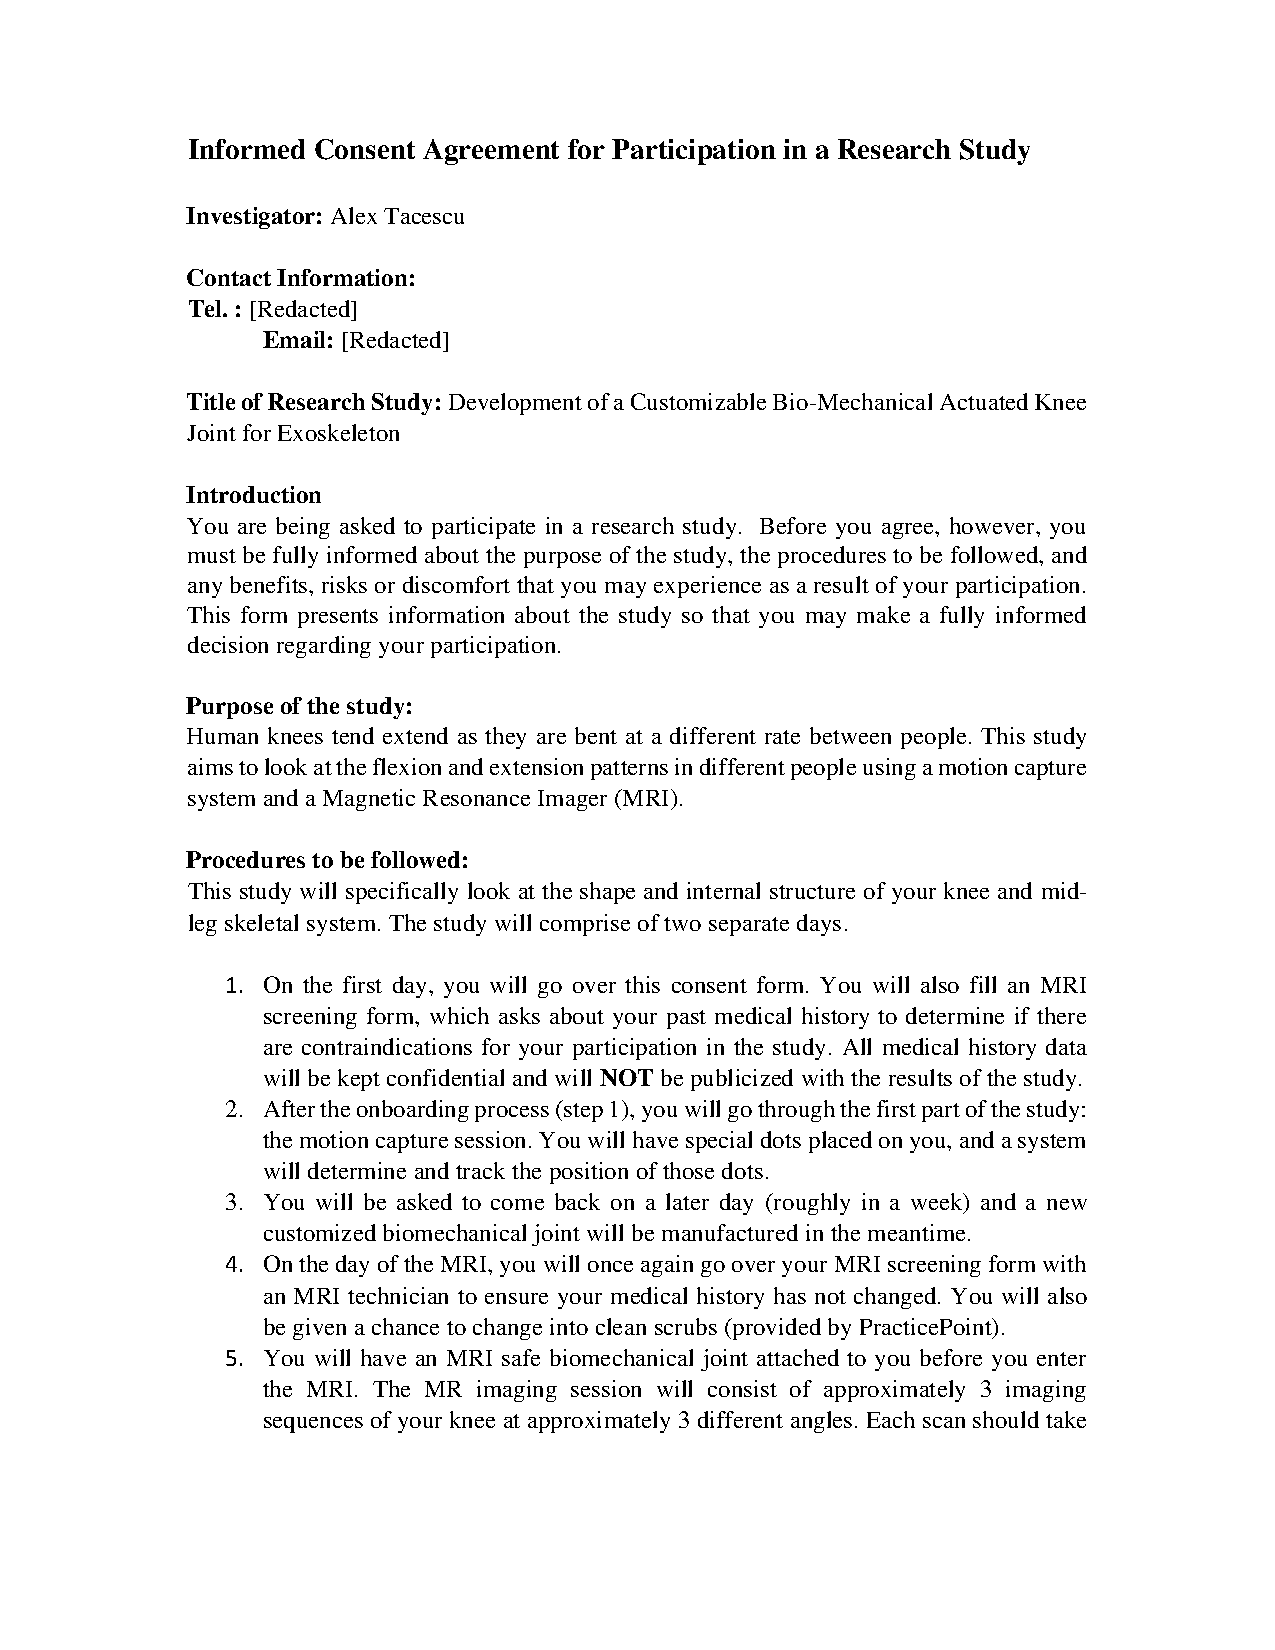
\includepdf[]{Appendix/ConsentForm.pdf}